\subsection{Laravel, c'est quoi?}

\subsubsection[Prélude]{Prélude}

\laravel{}{} est ce qu'on appelle un \textit{framework}. C'est à dire un ensemble d'outil fournissant une architecture de base sur laquelle n'importe quel site web peut être bâti. A la fin de ce \textit{``petit''} tutoriel, vous serez je l'espère capable d'utiliser les fonctionnalités principales de Laravel, ainsi que les languages utilisés par ce framework et par la création de site web en général: \php{}, \html{} et en allant un petit peu plus loin, \css{}, \jquery{}  et \js{}. Cela parait beaucoup d'un coup, mais en y allant méthodiquement et pas à pas, ça devrait bien se passer!

Bon alors, et ce framework alors? Comment fonctionne-t'il?

\subsubsection[Fonctionnement et philosophie]{Fonctionnement \& philosophie}\label{sec:fonctionnement&philosophie}

\laravel{}{} utilise une architecture dite ``MVC'' (Modèle, Vue, Contrôleur) qui est décrite par la figure \textsc{Figure }\ref{fig:laravel_diagram}. Elle se base donc sur 4 concepts:
\begin{enumerate}
    \item \texttt{Routing:} Le routing est l'étape consistant à lier une URL, une \route{}, à une action spécifique, qui sera effectuée par une méthode (dans le sens \textit{Object-oriented-programming} du terme) contenue dans un \controller{}.
    \item \texttt{Controller:} Les \controllers{} sont donc appellés par les \texttt{routes}, ce sont eux qui vont s'occuper de manipuler les données, effectuer x-y-z tâches, et enfin d'envoyer une certaine \view{} à l'utilisateur.
    \item \texttt{View:} Le concept de \view{} est plutôt simple: Avec Laravel, chaque view correspond grosso-modo à une page que l'utilisateur voit affichée sur son écran.
    \item \texttt{Model:} Enfin, les données stockées dans la base de donnée ne sont pas traitées telles quelles. Laravel nous facilite la vie en associant chaque type de donnée à un \model{}, qui sera plus simple à utiliser par les \controllers{} et comportera des fonctionnalités très utiles.
\end{enumerate}

\begin{figure}[!h]
    \centering
    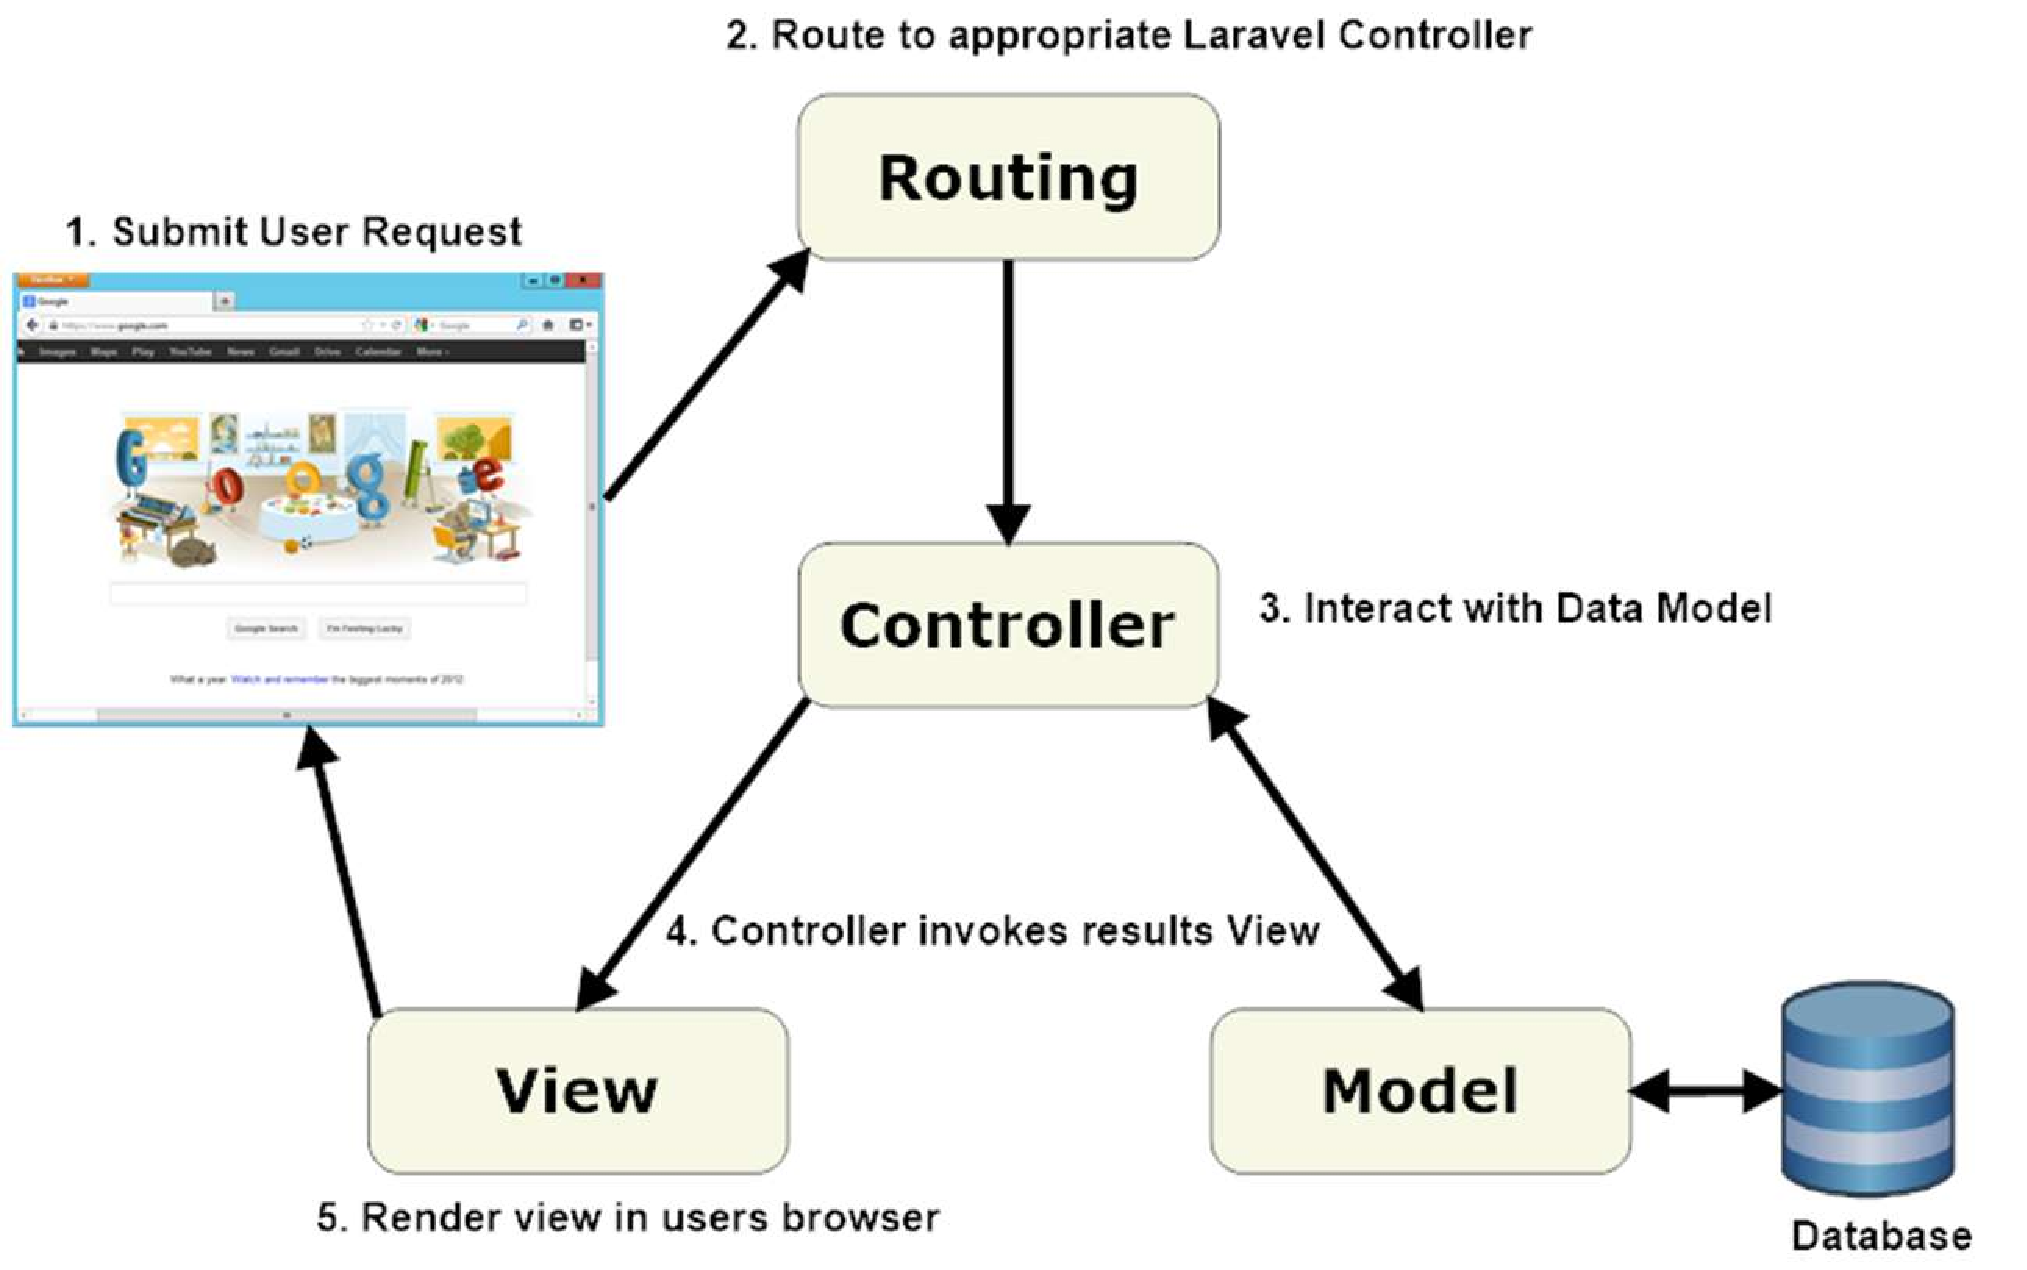
\includegraphics[width=0.5\textwidth]{figures-C1/diagram.pdf}
    \caption{\label{fig:laravel_diagram}}
\end{figure}